\subsubsection{Kubernetes Architecture}

As described by \cite{brendan_tracey_2018}, although Kubernetes' conception makes it easier to deploy and manage distributed systems, Kubernetes itself is a distributed system that needs to be managed. Its architecture/cluster can be divided into two layers: the control plane and the worker plane, as seen in figure \ref{fig:k8s-arch}. Kubernetes \citeonline{kubernetes_components_2019} call these components as key to make up a K8S cluster. Given the importance of these architectural elements, it is necessary to delve into the details regarding these two components. 

\begin{figure}[ht]
    \centering
    \caption{Kubernetes Architecture}
    \label{fig:k8s-arch}
    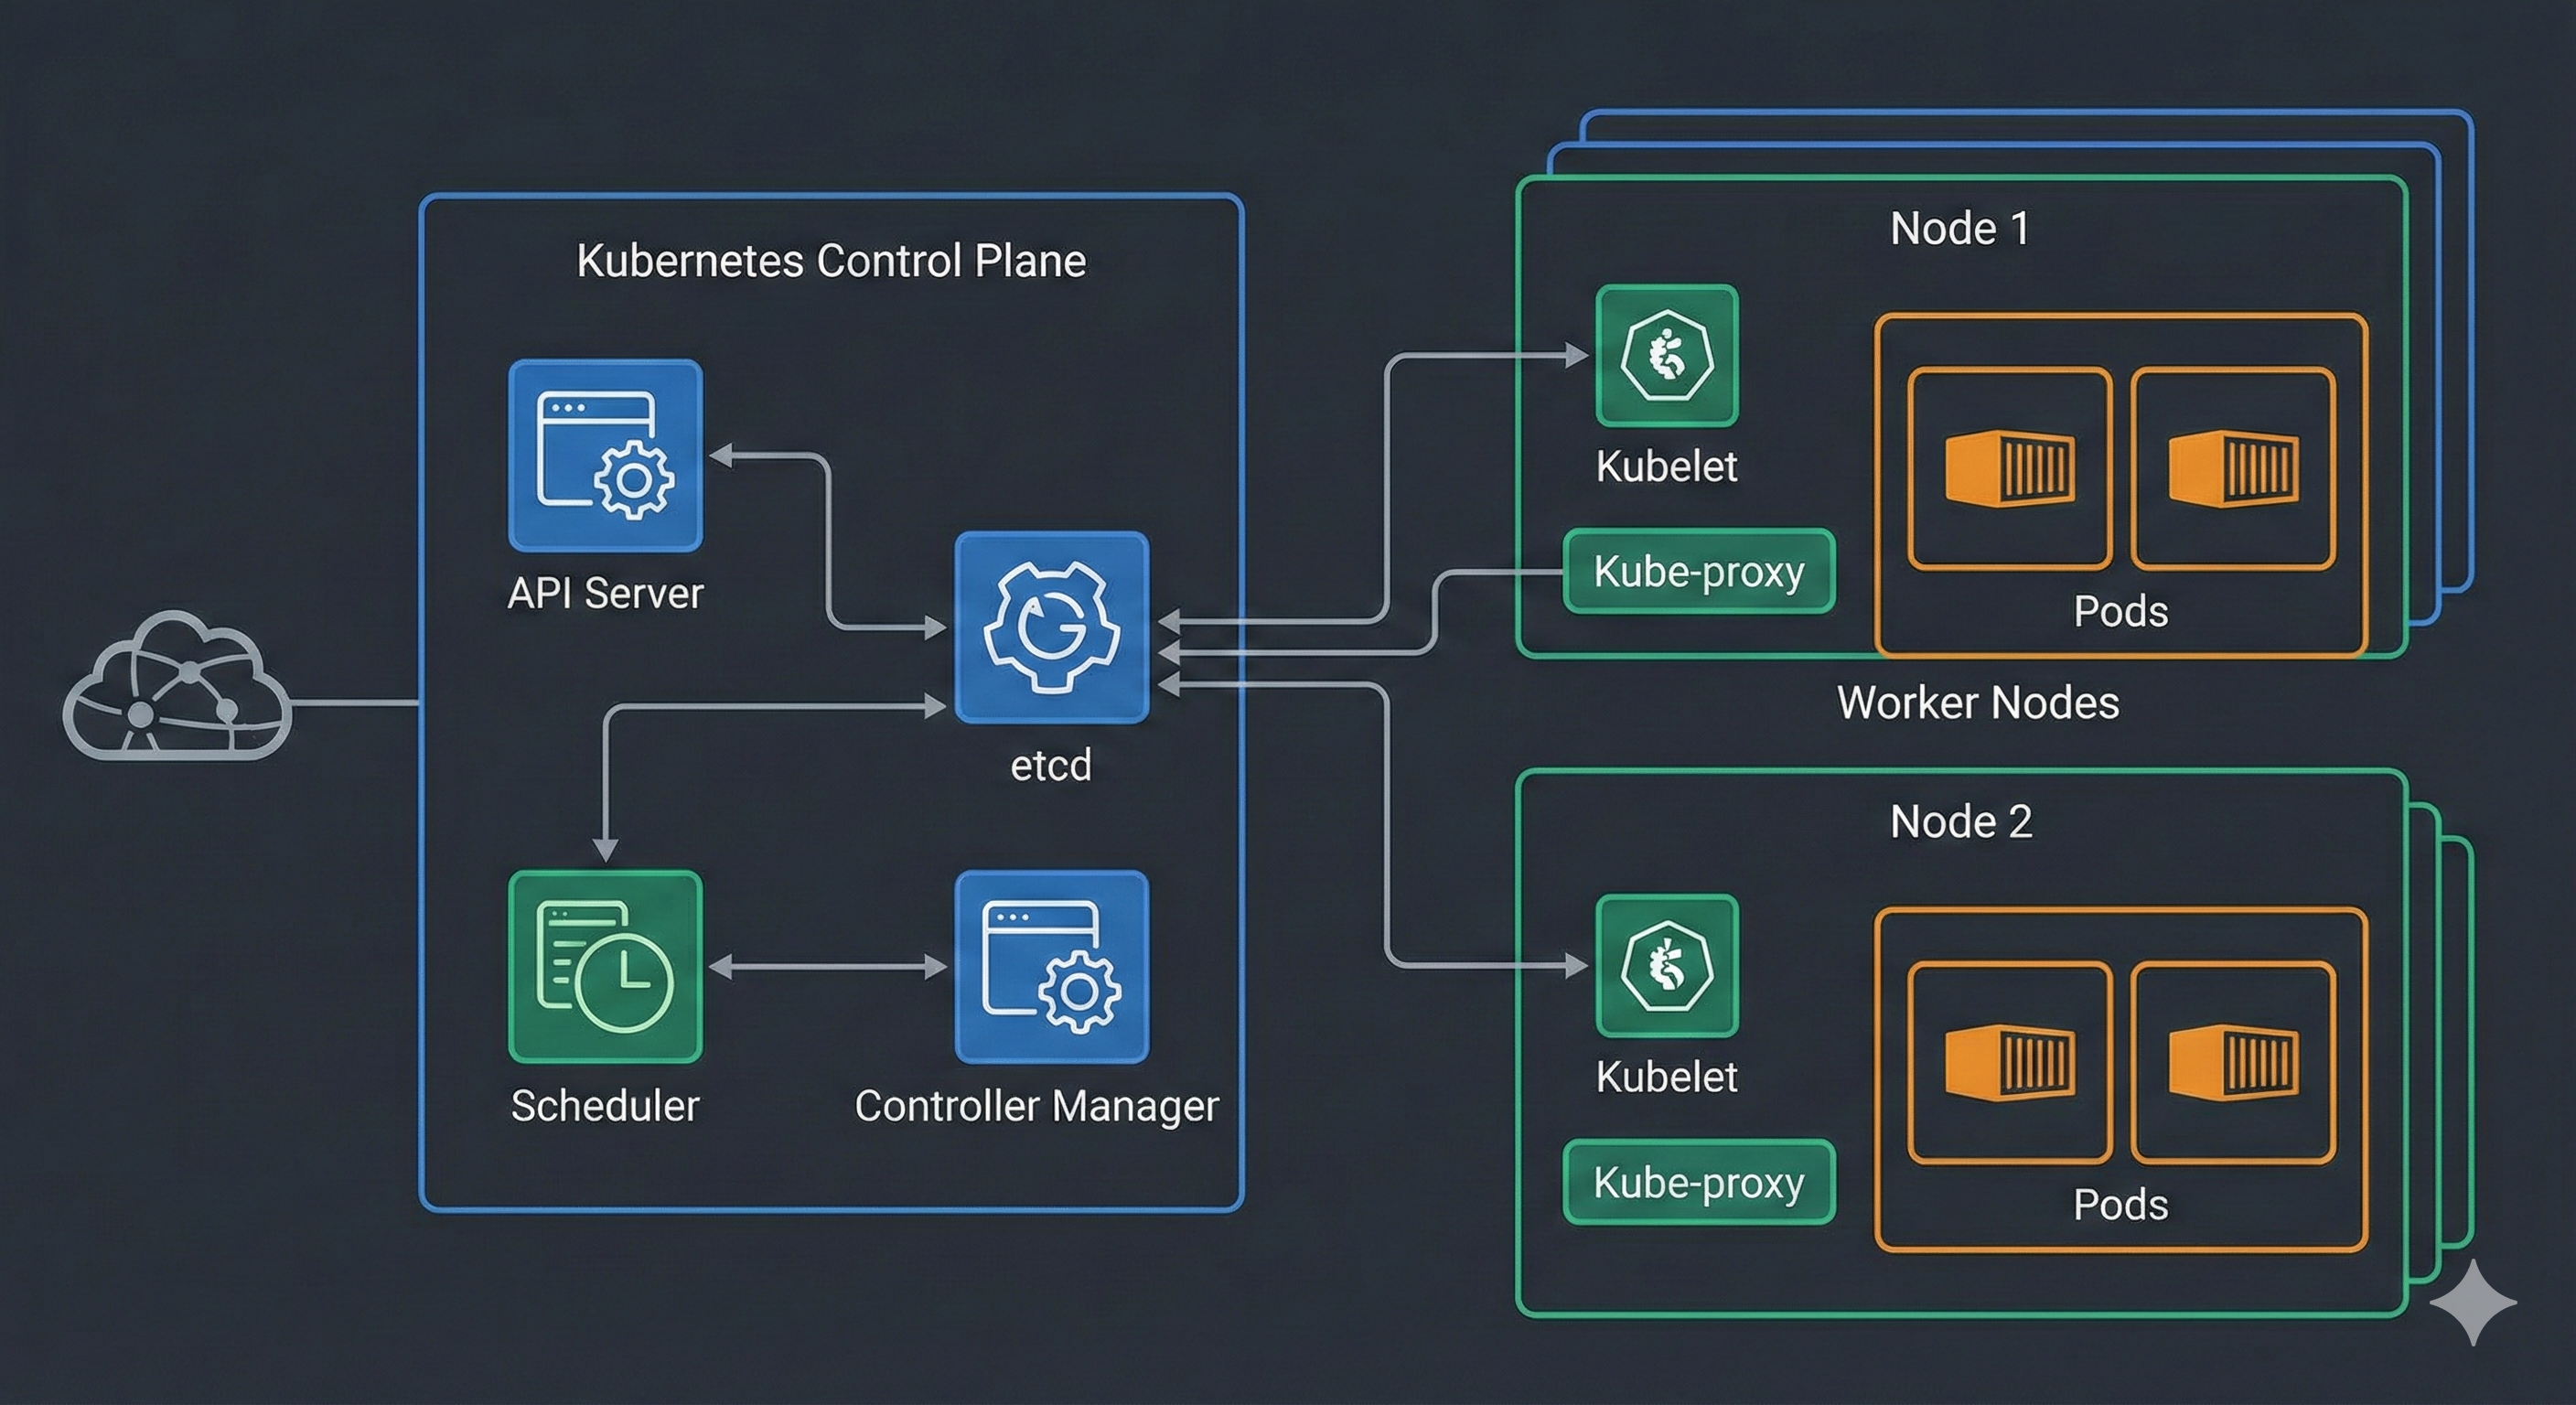
\includegraphics[width=1.0\linewidth]{images/cloud-computing/k8s-architecture.png}
    \par\medskip\ABNTEXfontereduzida\selectfont\textbf{Source:} \cite{kubernetes_2019} \par\medskip
\end{figure}

\textbf{The Control Plane}

The Control Plane is what controls the cluster and makes it function \cite{luksa_2018}. It is known as the ``brain'' of the cluster \cite{brendan_tracey_2018}. It is responsible for making global decisions (such as scheduling), detecting and responding to events (such as starting a new Pod when a replica fails), and maintaining the desired state of the system. In standard architecture diagrams (figure \ref{fig:control-plane}), it is often represented as a block containing four essential components and one optional:

\begin{figure}[ht]
    \centering
    \caption{Control Plane}
    \label{fig:control-plane}
    \includegraphics[width=1.0\linewidth]{images/cloud-computing/control-plane.png}
    \par\medskip\ABNTEXfontereduzida\selectfont\textbf{Source:} \cite{kubernetes_2019} \par\medskip
\end{figure}

\begin{itemize}
    \item API Server: The central component and the only communication interface for the Control Plane. All other components (whether the Scheduler, the Controller Manager, or the Kubelet on the nodes) communicate solely with the API Server, never directly with each other or with the database. It validates and configures data objects (Pods, Services, etc.).
    \item etcd: This is the consistent, high-availability key-value store used as the "source of truth" (backing store) for all cluster data. Kubernetes does not store state in the processing components; everything is persisted in etcd. Only the API Server has permission to read from and write to it.
    \item Scheduler: The component is responsible for resource allocation. It watches for newly created Pods that do not yet have a Node assigned and selects the best Node for them to run on, based on resource constraints (CPU/Memory), affinity policies, taints, and tolerations.
    \item Controller Manager: This component executes the control loops. It monitors the cluster's current state via the API Server and compares it with the desired state. If there is a divergence (e.g., a Pod died and the desired state specifies 3 replicas), it takes steps to correct it (e.g., creating a new Pod). It includes controllers such as the Node Controller and the Replication Controller.
    \item Cloud Control Manager: The component is responsible for integrating with cloud providers such as GCP \cite{kubernetes_components_2019}.
\end{itemize}

\textbf{Worker Nodes}

The Worker Nodes (represented as Node 1 and Node 2 in typical diagrams) are the "muscles" of the cluster. These are the machines (physical or virtual) where the workloads (applications) actually run. Each node has components to manage containers and communicate with the Control Plane:

\begin{itemize}
    \item Kubelet: The primary agent running on each node. It registers the node with the API Server and watches for Pod specifications (`PodSpecs`) assigned to that node. The Kubelet ensures that the containers described in those Pods are running and healthy, reporting their status back to the Control Plane. It also interacts with native monitoring tools, such as cAdvisor, to collect usage metrics.
    \item Kube-proxy: A network proxy running on each node. It maintains network rules (using `iptables' or `ipvs' on Linux) to allow network communication to Pods from within or outside the cluster. It enables the concept of a "Service" in Kubernetes by performing basic load balancing.
    \item Pods: Often represented as blocks containing containers, Pods are the smallest deployable unit in Kubernetes. A Pod encapsulates one or more containers (usually Docker/containerd), shared storage, and a unique IP within the cluster network.
\end{itemize}

\textbf{The Master-Worker Relationship}

The relationship between the Control Plane (historically called the Master) and the Worker Nodes is one of Command and Execution:

Unlike imperative orchestration models that rely on direct, synchronous execution of commands, the interaction between the Kubernetes Control Plane and Worker Nodes is fundamentally declarative and asynchronous \cite{burns_2016}. In this paradigm, the Control Plane does not micromanage individual node operations; instead, it persists the \textit{desired state} of the system into etcd, which serves as the single source of truth \cite{luksa_2018}.

The orchestration process follows a rigorous reconciliation loop:

\begin{enumerate}
    \item Scheduling: The \textit{kube-scheduler} evaluates resource constraints and affinity policies to assign (bind) a pending Pod to a specific Node, updating the API Server record \cite{hausenblas_2023}.
    \item Actuation: The \textit{Kubelet} daemon does not passively wait for commands. Instead, it utilizes a Watch API mechanism to continuously monitor the API Server for new specifications assigned to its node. Upon detecting a state divergence (e.g., a new Pod assignment), the Kubelet instructs the local container runtime (CRI) to align the actual state with the desired specification \cite{sayfan_2017}.
    \item Self-Healing: System resilience is maintained through continuous monitoring. If a node fails to renew its lease (heartbeat), the \textit{kube-controller-manager} detects the deviation from the desired state and automatically reschedules affected workloads to healthy nodes, ensuring state convergence without human intervention \cite{beyer_2016}.
\end{enumerate}

This separation ensures that the orchestration intelligence (Control Plane) is decoupled from the actual workload (Worker Nodes), allowing the system to be highly scalable and resilient.